\chapter[In memory of Professor G Ramachandran]{In memory of\\ Professor G Ramachandran}\label{chap28}

\Authorline{A R Usha Devi\footnote[*]{Email: \url{ushathirthahalli@gmail.com}}}
\addtocontents{toc}{\protect\contentsline{section}{{\sl A R Usha Devi}\smallskip}{}}
\authinfo{Professor, Physics Department, Bangalore University}

\renewcommand{\thefootnote}{\arabic{footnote}}

I cannot believe that Professor G. Ramachandran is no more and I am writing this in his memory! On 9th April 2020 I received a phone call from Professor K. S. Mallesh around 9 PM, informing me that Prof.\ G. Ramachandran passed away after suffering a massive heart attack. A shocking news - Professor G. Ramachandran was strong and energetic till this unexpected end. It is a difficult reality to come to terms with.
\vskip 2pt

Professor G. Ramachandran (fondly referred to as GR by his students) inspired many students by his vast knowledge, sharp intellect and his child like enthusiasm. GR shaped my thinking, my views on life and my work during the years 1988-1998 that I spent in the Department of Studies in Physics, Manasagangotri, University of Mysore, Mysore (as a M.Sc.\ student during 1988--90 and as a Ph.D. student under GR’s supervision during 1991-98).
\vskip 2pt

I vividly recall my first interaction with GR during late 1988. GR did not teach any course during our Junior M.Sc.\ We had heard a lot of appreicating remarks about GR from our senior students. A group of four students, including me and my sister Sudha, wanted to meet GR, though we did not know how to approach him! One fine day we saw GR standing alone outside his chamber. We decided to go and talk to him. I told GR ``We are very much interested in theoretical physics and want to get some exposure from you on this." GR warmly welcomed us into his office and started conversing casually. He began describing (for around 2 hours) Dirac’s relativistic quantum theory (which we had not studied in our first year M.Sc.) and went on to explain several subtleties of quantum field theory. For us, it was like “Alice in the wonderland” experience. We were spell-bound during GR's inspiring narrative. We missed our lunch in the hostel that day - never mind - we decided to take up theoretical physics as our special subject. Unfortunately only six students opted for this special subject at the end of the academic year 1988--89 and we were told that theoretical physics is not going to be offered; we had to alter our choice. It was indeed a helpless situation. But both GR and Professor A. V. Gopal Rao (AVG) encouraged us to continue interacting with them on specific topics of theoretical physics. Sudha and me used to join discussions of GR's research group, where Professors Mallesh, Swarnamala Sirsi, Sandhya, Sudha Rao used to work out details of their research work on the black board; GR's sharp remarks, his eye for details made us realize for the first instance what a critical thinking is all about. We did not understand much during these discussions. But we were keen to develop our interest in the research topics being discussed and \textit{see} their intricate subtleties.
\vskip 2pt

GR taught us ``Advanced quantum mechanics" during our senior M.Sc.\ year. His relativistic quantum theory classes were remarkable. GR's grasp of physics awed and inspired me simultaneously. I used to note down every word GR used to utter (including his remarks like \textit{``this was another feather in the cap of Mr. Pauli"} - in the context of explaining Dirac's \textit{(negative energy sea)} in his class and most of my classmates teased me for that! During my senior M.Sc.\ year I chose the topic `Pion-Nucleon scattering experiments" for my seminar. GR took me through a detailed excursion on this topic. I fondly remember his powerful description laced with wonderful anecdotes and his enormous patience when I raised silly questions. I always wondered how a sequence of relevant thoughts used to emerge so effortlessly when GR spoke. Before the end of my second year M.Sc.\ I asked GR if I can work for my Ph.D. under his supervision. GR readily agreed. I got qualified under UGC-CSIR National Level Entrance Examination during 1991 and I joined the Department of Studies in Physics as a Junior Research Fellow.
\vskip 2pt

I should highlight an important observation here: When I started working with GR during early 1991, there were already four women research scholars (Dr.\ Sandhya, Dr.\ Sudha Rao, Dr.\ Swarnamala Sirsi and Dr.\ Vidya). working for their Ph.D. under his supervision. I don't know if this made it easy for me to approach GR; obviously GR did not have any gender bias while choosing students (which indeed happens to be an additional feather in GR's cap). All that mattered to him was our interest and dedication to work on theoretical physics. I always felt comfortable to discuss with GR. I realize that many theoretical physicsists of 90's had a preference to work with male students. I am indeed very grateful to GR for giving me an opportunity to work with him.
\vskip 2pt

I started working on the multiaxial decomposition of Cartesian tensors - as an initial exercise. This gave me an exposure to Majorana's 1935 paper on the decomposition of spin-\textit{j} state into 2\textit{j} constituent\break spinors. I realized the significance of Majorana geometric respresentation for pure symmetric multiqubit states (pure spin-\textit{j} states) in the field of quantum information processing in recent years. I am grateful to GR for imparting his expertise on angular momentum techniques. I have continued to work on permutation symmetric multiqubit systems, where angular momentum algebra serves as a powerful tool. My collaboration with Professor A. K. Rajgaopal (AKR) began in cyber space, when he wrote an email during 2005, appreciating my paper on the characterization of entanglement in symmetric qubit systems (in which the results were developed using angular momentum theory). AKR raised a very pertinent question on the impact of time-reversal on the two- qubit covariance matrix, which I could not address immediately. I realized its importance two months later and I wrote back to AKR. This marked the beginning of my ongoing research collaboration and a warm friendship with AKR. He appreciates my use of angular momentum methods in different research problems we have worked together (in fact AKR calls it a \textit{gold mine} that I own. I owe it to GR, for shaping my thoughts). AKR continues to keep pointing out research developements on symmetric multiqubit systems and on the applications of Majorana geometric representations\footnote{Sudha has contributed an article on \textit{The Majorarana  geometric representation of pure symmetric multiqubit states} (authors: Sudha, A. R. Usha Devi and A. K. Rajagopal) to this volume.}; collaborates with me to continue working enthusiastically on a wide range of topics in the field of quantum information theory. During one of his visits to India (and Bengaluru) in 2007, AKR said he would like to meet GR. The photograph featuring three of us is captured when we visited GR at his Jayanagar residence. I recall that GR spoke enthusiastically about his new thoughts on polarization phenomena in astrophysics during this meeting. He was glad to learn about my work with AKR.
\newpage

\begin{figure}[H]
\centering
\includegraphics[scale=0.21]{src/images/chap18/001.eps}
\caption{Photograph taken during 2007:\\ GR, AKR and Usha}\label{chap18-fig001}
\end{figure}

I worked on \textit{inverse scattering} problem in the inelastic scattering of protons on $^{12}{\rm C}$ target nucleus with my senior collegue Professor Sudha Rao for two years. I was somehow not enthusiastic to continue on this. Eventually, during the third year, I developed interest towards foundations of quantum theory (once again it was GR's description of EPR paradox on the one hand and his interest in quasi-probability distributions in quantum theory on the other hand, which motivated me). I started working with my senior colleague Professor Swarnamala Sirsi on Wigner’s phase space formalism in quantum theory. I have evergreen memories of our enthusiastic disucssions with GR in the verandah of his residence (almost every evening - starting around 4 pm to around 9 pm). I had developed a suitable unitary transformation, which helped us in simplifying the Wigner-Weyl characteristic function. GR had casually referred to it as ``U(sha) transformation". His encouragement on my little contributions indeed helped me carry on with increased enthusiasm. One of those days, GR informed us that he had a discussion with KRP (Professor K. R. Parthasarathy, with whom GR had his association at Indian Statistical Institute, Calcutta) on the properties of moments of a legitimate probability distribution. We discussed at a great length on how these properties are violated in the example of spherical tensor moments $\langle T_{q}^{k} \rangle$, when non-commuting angular momentum components replace the conventional random variables of classical probability theory. This invoked great interest in me to pay attention to the rigorous theory of quantum probability. During the year 2016-17 I took sabbatical leave from Bangalore University and worked with KRP\footnote{Prof.\ K. R. Parthasarathy recollects his association with GR: ``Professor G. Ramachandran joined Indian Statistical Institute, Calcutta as a faculty, during 1960's. We used to stay in the Institute hostel for some time (before Ramachandran's family moved to Calcutta). I distinctly remember that Ramachandran was looking for a house, with a Well, in the Baranagar area of Calcutta. During this period I was busy with my research work on information theory, but we had occasional discussions where GR had shared some of his ideas on the density operators in quantum theory. When I had visited Mysore to deliver a series of lectures at the mathematics and the statistics departments of University of Mysore, G. Ramachandran had invited me for dinner at his residence. On that occasion we had an elaborate discussion on various aspects of quantum theory. I was served a sumptuous traditional meal on a plantain leaf at G. Ramachandran's house. Two of GR’s students, V. Ravishankar and A. R. Usha Devi worked with me at the Indian Statistical Institute, Delhi during later years."} at the Indian Statistical Institute, Delhi center on quantum stochastic dynamics. It is KRP, who suggested that a comprehensive article on quantum state diffusion (on which I had worked with KRP during the period 2016-18) would be an appropriate contribution to the volume being brought out in GR’s memory.

I am indebted to GR for directing me to several rare and precious books and research papers during the early years of my research: \textit{Theory of angular momentum} by M. E. Rose, \textit{Angular momentum in quantum physics} by L. C. Biedenharn and J. D. Louck, \textit{The physics of elementary particles} by H. Muirhead, \textit{Elementary particle physics} by S. Gasiorowicz, \textit{Advanced quantum theory} by Paul Roman, \textit{The unitary and rotation groups} by F. D. Murnaghan, \textit{The special theory of relativity} by J. Aharoni; \textit{Classical and quantum theories of spinning particles} by H. C. Corben, \textit{Quantum electrodynamics} by G. K\"{a}llen, books and papers by A. O. Barut, R. H. Good Jr,... to mention a few.

GR's motto: ``the pursuit of science is best done when it becomes a way of life" would always remain as a great source of inspiration for me to carry on....
\vskip 0.5cm

%~ \centerline{\includegraphics[scale=1]{authorsphotos/Prof_A_R_Usha_Devi.eps}}
%~ \medskip

%~ \noindent
%~ \textbf{Dr.\ A. R. Usha Devi} obtained the M.Sc.\ degree in 1990 and Ph.D. in 1998 from Mysore University. She worked for Ph.D. under the guidance of Prof.\ G. Ramachandran. Currently she is a Professor of Physics at Bangalore University.

%~ \noindent
%~ \begin{minipage}[t]{4cm}%
%~ \phantom{i}\\[-1.5cm]%
%~ \includegraphics[scale=0.85]{authorsphotos/Prof_A_R_Usha_Devi.eps}
%~ \end{minipage}\quad
%~ \begin{minipage}{5cm}
%~ \textbf{Dr.\ A. R. Usha Devi} obtained the M.Sc.\ degree in 1990 and Ph.D. in 1998 from Mysore University. She worked for Ph.D. under the guidance of Prof.\ G. Ramachandran. Currently she is a Professor of Physics at Bangalore University.
%~ \end{minipage}
